\documentclass[a4paper,10pt]{article}

\usepackage[utf8]{inputenc}
\usepackage{t1enc}

\usepackage[utf8]{inputenc}
\usepackage{t1enc}
\usepackage[spanish]{babel}
\usepackage[pdftex,usenames,dvipsnames]{color}
\usepackage[pdftex]{graphicx}
\usepackage{enumerate}
\usepackage{amsmath}
\usepackage{amsfonts}
\usepackage{amssymb}
\usepackage[table]{xcolor}
\usepackage[small,bf]{caption}
\usepackage{float}
\usepackage{subfig}
\usepackage{listings}
\usepackage{bm}
\usepackage{times}
\usepackage{marvosym}


\begin{document}
\setcounter{secnumdepth}{5}
\setcounter{tocdepth}{5}

\renewcommand{\lstlistingname}{C\'odigo Fuente}
\lstloadlanguages{Octave} 
\lstdefinelanguage{MyOctave}[]{Octave}{
        deletekeywords={beta,det},
        morekeywords={repmat}
} 
\lstset{
        language=MyOctave,
        stringstyle=\ttfamily,
        showstringspaces = false,
        basicstyle=\footnotesize\ttfamily,
        commentstyle=\color{gray},
        keywordstyle=\bfseries,
        numbers=left,
        numberstyle=\ttfamily\footnotesize,
        stepnumber=1,                   
        framexleftmargin=0.20cm,
        numbersep=0.37cm,              
        backgroundcolor=\color{white},
        showspaces=false,
        showtabs=false,
        frame=l,
        tabsize=4,
        captionpos=b,               
        breaklines=true,             
        breakatwhitespace=false,      
        mathescape=true
}

%%%%%%%%%%%%%%%%%%%%%%%%%%%%%%%%%%
%%%%%%%% begin TITLE PAGE %%%%%%%%
%%%%%%%%%%%%%%%%%%%%%%%%%%%%%%%%%%
\begin{titlepage}
        \vfill
        \thispagestyle{empty}
        \begin{center}
                
\includegraphics{./images/itba_logo.png}
                \vfill
                \Huge{Sistemas de Inteligencia Artificial}\\
                \vspace{1cm}
                \Huge{Redes Neuronales}\\
                \vspace{1cm}
                \Huge{Trabajo Pr\'actico Especial 2}\\
        \end{center}
        \vfill
        \large{
        \begin{tabular}{lcr}
                Civile, Juan Pablo && 50453\\
                Ordano, Esteban && 50753\\
                Crespo, Alvaro && 50758 \\
        \end{tabular}
}
        \vspace{2cm}
        \begin{center}
                \large{24 de abril de 2013}\\
        \end{center}
\end{titlepage}
\newpage

\setcounter{page}{1}

% \tableofcontents
% \newpage

\section{Definición del problema}

El problema consiste en la implementación de una red neuronal multicapa con aprendizaje supervisado que realice la predicción de series temporales. Para ello se supone que $x(t)$ (el valor de la 
serie en el paso temporal $t$) es alguna función desconocida de los valores de la serie en pasos anteriores, es decir, $x(t) = f (x(t - 1), x(t - 2), x(t - 3), \dots)$. 
La red neuronal deberá poder aproximar a la función $f$ desconocida. No se
conoce la cantidad de valores anteriores de la serie respecto a los cuales $f$ es función.

\section{Implementación}

    Se implementó una red multicapa de tipo \texttt{Feed Forward}, usando el
    algoritmo \texttt{Back Propagation} para el entrenamiento de la misma.
    La distribución inicial de pesos se generó de manera aleatoria con valores
    acotados a un intervalo dependiente de la función de activación en uso.
    Como medida del error se usó la función de error cuadrático medio.

    \subsection{Funciones de activación}
    Se utilizaron las siguientes funciones de activación y sus respectivas derivadas:

    \begin{itemize}
        \item Función Sigmoidea
            \[ g(x) = \dfrac{1}{1 + exp^{-x}} \]
            \[ g'(x) = \dfrac{1}{(-2 * cosh(x) - 2)}\]
        \item Tangente hiperbólica
            \[ g(x) = tanh(x) \]
            \[ g'(x) = sech(x)^{2} \]
    \end{itemize}

    \subsection{Normalización de la entrada y la salida}

        Dado que las entradas y salidades de la red pertenecen al intervalo $(-4, 4)$, y las entradas y las salidas de las funciones de activación utilizadas 
        pertenecen al intervalo $(0,1)$ para el caso de la sigmoidea, y al $(-1,1)$ en el caso de la tangente hiperbólica, se debe realizar una normalización 
        tanto en la entrada como en la salida de la red. Estas normalizaciones son las siguentes:

        \begin{itemize}
            \item Sigmoidea

                Para la entrada: \[ \xi_{i} = \frac{x_{i} + 4}{8} \]
                Para la salida: \[ o_{i} = x_{i} * 4 \]
            \item Tangente hiperbólica

                Para la entrada: \[ \xi_{i} = x / 4 \]
                Para la salida: \[ o_{i} = (x - 0.5) * 8 \]
        \end{itemize}

    \subsection{Mejoras}

        \subsubsection{Momentum}

        Momentum considera los valores de $\Delta w_{ij}$ de pasos anteriores a la hora de actualizar los pesos del paso actual.
        En particular, se agrega al cambio dado por \texttt{Back Propagation}, el cambio de la iteración anterior pesado por un factor $\alpha$.

        \subsubsection{$\eta$ adaptativo}

        Esta mejora busca alterar el valor de $\eta$ de acuerdo al progreso del entrenamiento.
        Para esto se considera que si se encuentra una secuencia de $k$ pasos que disminuyen el error, entonces se tiene un buen camino de entrenamiento y por lo tanto se aumenta 
        el valor en una constante $a$ para continuar avanzando en este sentido.
        Y si por el contrario se encuentra en un mal camino, se disminuye el valor en un porcentaje $b$.
        Cuando se disminuye el valor, se desactiva temporalmente la mejora \texttt{Momentum} y se descarta el paso realizado.
        Una vez que se encuentra un paso que disminuye el error se reactiva la
        estrategia de \texttt{Momentum}.

        \subsubsection{Ruido}

        Se intentó introducir ruido a los pesos de la red entre pasos para
        evitar caer en mínimos locales.
        Se agregó a cada peso un valor aleatorio entre 0 y 1, adjustado por la
        cantidad de \textit{rollbacks} (entrenamientos que se descartaron por no
        disminuir el error), y una constante.
        Esta optimización fue descartada porque en manera consistente no
        mejoraba los resultados obtenidos.

    \subsection{Conjunto de entrenamiento y prueba}

    Se tiene un conjunto de 1000 puntos de la serie a ser generalizada.
    Para el entrenamiento de la red se utilizaron los primeros 800 puntos,
    y los restantes 200 puntos fueron utilizados como conjunto de prueba.
    Siempre que se habla del error medio de una red, se refiere al error
    cuadrático medio del conjunto de prueba.

    \subsection{Disminución de la cantidad de entrenamientos descartados}
        \label{less_rollbacks}
        Se consideró incorporar otros criterios para deshacer entrenamientos utilizando la estrategia de entrenamiento adaptativo. Además de considerar el error cuadrático medio, 
        se consideró como un valor relevante el de un percentil alto (se seleccionó el percentil $90$) de los errores del conjunto de entrenamiento. El objetivo es no descartar 
        entrenamientos que son mejores, aunque el error medio no disminuya. Dos
        nuevos criterios utilizando este nuevo parámetro son no realizar
        \textit{rollback} si:

        \begin{itemize}
            \item Disminuye el error cuadrático medio \textbf{y} disminuye el percentil 90.
            \item Disminuye el error cuadrático medio \textbf{o} disminuye el percentil 90.
        \end{itemize}

    \subsection{Selección de los parámetros de configuración}

        \label{sec:configuracion}
        El entrenamiento de la red neuronal con las estrategias implementadas tiene una extensa variedad de parámetros de configuración. Además de $\eta$, 
        el coeficiente de aprendizaje, el entrenamiento con la estrategia \textit{Momentum} requiere seleccionar un valor para $\alpha$, el término que pesa el descenso promedio. 
        La estrategia de entrenamiento adaptativo requiere la selección de más parámetros: los factores $a$, $b$, y la cantidad de pasos $k$.
        Se determinaron valores iniciales que producían resultados suficientemente satisfactorios en 1500 iteraciones. Se consideró cada parámetro independientemente de los demás y se iteró por valores relevantes para cada variable.

\section{Resultados y Conclusiones}

    \subsection{Comparación de Funciones de Activación}
    \label{sec:comparacion-activacion}

    Para realizar una comparación entre las funciones de activación utilizadas,
    se definió un set de arquitecturas de prueba de manera arbitraria.
    Para esta comparacion, se mantuvieron fijos los parámetros de entrada de la
    red y se limitó la cantidad de iteraciones a 1500.
    Según la función de activación usada en cada caso, se acotaron los valores
    aleatorios de los pesos utilizados como entrada al algoritmo de aprendizaje
    supervisado. Como era de esperarse, para la función sigmoidea, hubo que
    generar números muy pequeños en módulo (cercanos a 0), para que no se saturen
    las conexiones, y se impida el aprendizaje.
    Para el caso de la tangente hiperbólica, en cambio, esos pesos iniciales
    pequeños no retornaron resultados positivos, como si lo hicieron las pruebas
    realizadas con valores aleatorios pero con cotas mayores.

     \begin{table}[H]

        \begin{center}
        \begin{tabular}{|l|r|r|}
            \hline
            Arquitectura \textbackslash Función de activación & Tangente hiperbólica & Sigmoidea \\
            \hline
            [2 5 4 1] & $0.023053$ & $0.31491$ \\
            \hline
            [3 10 6 1] & $0.053163$ & $0.30446$  \\
            \hline
            [2 10 6 1] & $0.029276$ & $0.31163$  \\
            \hline
            [2 4 2 1]  & $0.36896$ & $0.31504$  \\
            \hline
            [3 14 8 1] & $0.028585$ & $0.30841$  \\
            \hline
        \end{tabular}
        \end{center}
        \caption{Comparación del error cuadrático medio entre las funciones de activación \textit{Tangente hiperbólica} y \textit{Sigmoidea}.}
        \label{table-comparation-act-functions}

    \end{table}

    Se observa en \label{table-comparation-act-functions} que las redes obtenidas con la función $tanh$ son ampliamente superiores a sus contrapartes con la función \textit{Sigmoidea}.
    A partir de este resultado, se prosiguió el análisis en redes construidas con la función \textit{tangente hiperbólica}.

    \subsection{Optimización de parámetros}
    \label{sec:parametros-optimos}

        Se muestran los resultados obtenidos de la selección descripta en la sección \ref{sec:configuracion} para cada variable en la tabla \ref{tabla_configuracion}. 
        Al respecto, se hacen las siguientes observaciones:

        \begin{itemize}
        \item El mejor valor para el coeficiente $alpha$ es de $0.3$, mucho
        menor que el sugerido $0.9$.
        \item El mejor valor del parámetro $a$ es de $0.0001$. Este valor es menor de lo esperado, ya que en pruebas preliminares un valor de $0.01$ 
              no arrojaba peores resultados que correr el algoritmo sin la estrategia de entrenamiento adaptativo.
        \item El mejor valor del parámetro $b$ es de $0.01$. Esto es mayor de lo esperado, el valor que se utilizaba inicialmente era de 0.001.
        \end{itemize}

        \begin{table}[H]
            \begin{tabular}{|c|c|c|c|c|}
                \hline
                Parámetro & Minimo valor & Incremento & Máximo valor & Mejor valor \\ \hline
                $alpha$ & $0.1$ & $+ 0.1$ & $0.9$ & $0.3$ \\ \hline
                $a$ & $0.00001$ & $\Cross 10$ & $0.01$ & $0.0001$ \\ \hline
                $b$ & $0.00001$ & $\Cross 10$ & $0.01$ & $0.01$ \\ \hline
                $k$ & $1$ & $+ 1$ & $5$ & $4$ \\ \hline
            \end{tabular}
            \caption{Parámetros de configuración de la red neuronal}
            \label{tabla_configuracion}
        \end{table}

        Con este analisis encontramos que los valores utilizados como parámetros
        en la sección \ref{sec:comparacion-activacion} resultaron muy cercanos a
        los óptimos.
        El unico parámetro con valor distinto es $a$ con un valor de $0.001$.

    \subsection{Estrategia de Rollback}

        Respecto a \ref{less_rollbacks}, la disminución de la cantidad de entrenamientos descartados, se puede ver que la estrategia de hacer rollback si el percentil 90 no disminuye consigue mejores resultados que la estrategia convencional y la estrategia de hacer rollback sólo si no disminuye la media y el percentil. Esto se puede ver en \ref{tabla_rollbacks}, donde este criterio mejora en un $25\%$.

    \begin{table}[H]
        \begin{tabular}{|c|c|c|c|c|}
        \hline
        Criterio & Rollbacks & $\overline{e_m}$ & $\overline{\sigma^2}$ & ${e_m}_{max} $ \\ \hline
        Solo la media & $507.5$ & $0.08498$ & $0.14161$ & $0.5671$ \\ \hline
        And & $476.6$ & $0.06458$ & $0.11795$ & $0.55802$ \\ \hline
        Or & $495.4$ & $0.09988$ & $0.17392$ & $0.76038$ \\ \hline
        \end{tabular}
        \caption{Criterio para descartar entrenamientos. Promedios obtenidos luego de 800 entrenamientos, sobre un conjunto de diez ejecuciones.}
        \label{tabla_rollbacks}
    \end{table}

    \subsection{Optimizarión de arquitectura}
    \label{sec:arquitectura-optima}

    Una vez conocidos los parámetros óptimos, se buscó optimizar la arquitectura utilizando estos valores.
    Para esto se corrieron repetidas ejecuciones de un abanico de arquitecturas de 2 entradas.
    No se utilizaron arquitecturas de 3 entradas ya que en la tabla \ref{table-comparation-act-functions} se observó que las redes de 3 entradas no presentan mejoras sustanciales sobre las de 2.

    Las arquitecturas que se consideraron tienen 2 capas ocultas.
    La siguiente figura muestra los menores errores obtenidos en estas
    ejecuciones para cada arquitectura. Se describe una arquitectura de $N$
    neuronas en la primer capa oculta y $M$ neuronas en la segunda capa oculta
    como una arquitectura de $NxM$.

    \begin{figure}[H]
        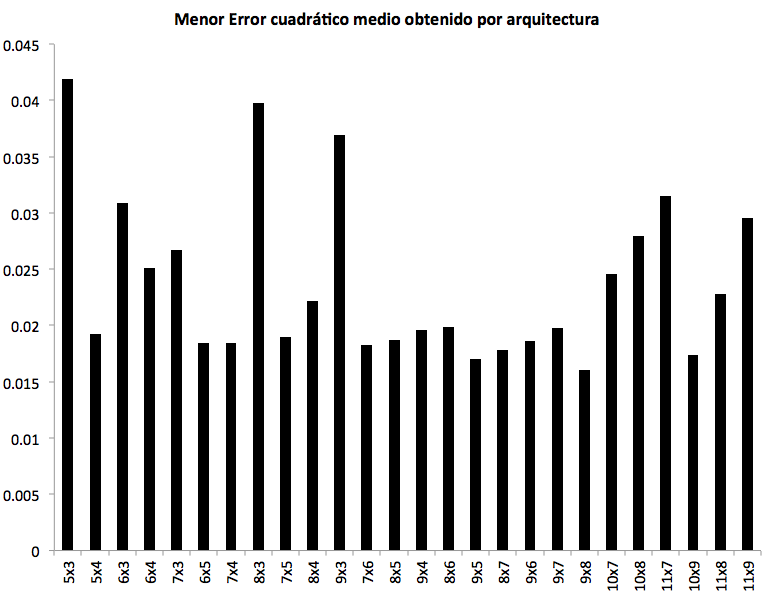
\includegraphics[scale=0.5]{./images/arquitecturas.png}
        \caption{Error cuadrático medio obtenido para arquitecturas con 2 entradas variando la cantidad de neuronas en la primera y segunda capa oculta}
        \label{fig:arquitecturas}
    \end{figure}

    De esta ejecucion pudimos obtener nuestra mejor red.
    Es la de arquitectura de 2 entradas, 9 neuronas en la primer capa oculta y 8 en la segunda capa oculta.
    Para esta red obtuvimos como error medio $0.01605$, una desviacion standard del error de $0.025738$ y un error maximo de $0.11786$.
    Se puede comparar este resultado con el resto de las arquitecturas en la tabla \ref{tab:arquitectura_full} en el anexo.

\section*{Anexo: Resultados}

\begin{table}[H]

\begin{tabular}{l|r|r|r|r}
Algoritmo & Tiempo (segs) & Estados & Expandidos & Frontera \\
\hline
DFS & 0.00301599502563 & 31 & 17 & 14 \\
BFS & 0.124269962311 & 472 & 472 & 0 \\
Iterative Deepening 3 & 0.125840902328 & 472 & 472 & 0 \\
Iterative Deepening 5 & 0.128756999969 & 472 & 472 & 0 \\
Greedy Ramas angostas & 0.00515198707581 & 31 & 17 & 14 \\
Greedy No eliminables & 0.00651216506958 & 63 & 17 & 46 \\
A* Ramas angostas & 0.135581016541 & 472 & 471 & 1 \\
A* No eliminables & 0.132388830185 & 472 & 472 & 0 \\

\end{tabular}
\caption{Mejor resultado del \textit{BFS} y \textit{A*}}
\label{crappy-best}

\end{table}

\begin{table}[H]

\begin{tabular}{l|r|r|r|r}
Algoritmo & Tiempo (segs) & Estados & Expandidos & Frontera \\
\hline
A* No eliminables & 21.61545286 & 100443.51 & 27311.39 & 73132.12 \\
A* Ramas angostas & 39.68114223 & 98606.65 & 27098.05 & 71508.6 \\
BFS & 20.0964277 & 100443.51 & 27361.04 & 73082.47 \\
DFS & 0.010342038 & 81.33 & 24.87 & 56.46 \\
Greedy Ramas angostas & 0.018111382 & 128.5 & 21 & 107.5 \\
Greedy No eliminables & 0.02189836 & 130.69 & 36.62 & 94.07 \\
Iterative 3 & 20.72738798 & 99684.76 & 26970.21 & 72714.55 \\
Iterative 5 & 21.6782024 & 100443.51 & 27361.04 & 73082.47
\end{tabular}

\caption{Promedio de los resultados de 100 ejecuciones}
\label{averages}

\end{table}



\end{document}
